\setcounter{section}{0}
\textbf{Định luật I Newton}

Nếu một vật không chịu tác dụng của lực nào hoặc chịu tác dụng tác dụng của các lực có hợp lực bằng không, thì vật đang đứng yên sẽ tiếp tục đứng yên, đang chuyển động sẽ tiếp tục chuyển động thẳng đều.

\textbf{Định luật II Newton}

Gia tốc của một vật cùng hướng với lực tác dụng lên vật. Độ lớn của gia tốc tỉ lệ thuận với độ lớn của lực và tỉ lệ nghịch với khối lượng của vật.
\begin{equation*}
	\vec{a}=\dfrac{\vec F}{m},
\end{equation*}
trong đó:
\begin{itemize}
	\item $\vec F$ là lực tác dụng lên vật (N);
	\item m là khối lượng của vật (kg);
	\item $\vec a$ là gia tốc của vật ($\text{m/s}^2$).
\end{itemize}

\textbf{Định luật III Newton}

Trong mọi trường hợp, khi vật A tác dụng lên vật B một lực, thì vật B cũng tác dụng lại vật A một lực. Hai lực này có cùng giá, cùng độ lớn, nhưng ngược chiều.
\begin{equation*}
	{\vec F}_{\text{AB}}=-{\vec F}_{\text{BA}}.
\end{equation*}
\section{Trắc nghiệm}
\begin{enumerate}[label=\bfseries Câu \arabic*:]
	\item \mkstar{1}
	
	
	{Định luật I Niu-tơn xác nhận rằng
		\begin{mcq}
			\item do quán tính nên mọi vật đang chuyển động đều có xu hướng dừng lại.
			\item với mỗi lực tác dụng đều có một phản lực trực đối.
			\item vật giữ nguyên trạng thái đứng yên hoặc chuyển động thẳng đều khi nó không chịu tác dụng của bất kì lực nào.
			\item khi hợp lực tác dụng lên vật bằng 0 thì vật không thể chuyển động được.
		\end{mcq}
	}
	
	\hideall
	{	\textbf{Đáp án: C.}
		
		Định luật I - Niu-tơn: Nếu một vật không chịu tác dụng của lực nào hoặc chịu tác dụng của các lực có hợp lực bằng không, thì nó giữ nguyên trạng thái đứng yên hoặc chuyển động thẳng đều.
		
	}
	
	\item \mkstar{1}
	
	
	{Hai lực trực đối cân bằng là hai lực
		\begin{mcq}
			\item tác dụng vào cùng một vật.
			\item không bằng nhau về độ lớn.
			\item bằng nhau về độ lớn nhưng không nhất thiết phải cùng giá.
			\item có cùng độ lớn, cùng phương, ngược chiều, tác dụng vào hai vật khác nhau.
		\end{mcq}
	}
	\hideall
	{	\textbf{Đáp án: D.}
		
		Hai lực trực đối cân bằng là hai lực có cùng độ lớn, cùng phương, ngược chiều, tác dụng vào hai vật khác nhau.
	}
	\item \mkstar{1}
	
	
	{Kết luận nào sau đây đúng?
		\begin{mcq}
			\item Nếu không có lực tác dụng vào vật thì vật không thể chuyển động được.
			\item Không cần có lực tác dụng vào vật thì vật vẫn có thể chuyển động tròn đều được.
			\item Lực là nguyên nhân duy trì chuyển động của một vật.
			\item Lực là nguyên nhân làm biến đổi chuyển động của một vật.
		\end{mcq}
	}
	
	\hideall
	{	\textbf{Đáp án: D.}
		
		Lực là nguyên nhân làm biến đổi chuyển động của một vật.
	}
	\item \mkstar{2}
	
	
	{Trường hợp nào sau đây có liên quan đến quán tính?
		\begin{mcq}(2)
			\item Vật rơi tự do.
			\item Vật rơi trong không khí.
			\item Chiếc bè trôi trên sông.
			\item Giũ quần áo cho sạch bụi.
		\end{mcq}
	}
	
	\hideall
	{	\textbf{Đáp án: D.}	
		
		Quán tính là tính chất của mọi vật có xu hướng bảo toàn vận tốc cả về hướng và độ lớn.
	}
	\item \mkstar{2}
	
	
	{Người ta dùng búa đóng một cây đinh vào một khối gỗ.
		\begin{mcq}
			\item Lực do đinh tác dụng vào búa lớn hơn lực do búa tác dụng vào đinh.
			\item Lực do đinh tác dụng vào búa nhỏ hơn lực do búa tác dụng vào đinh.
			\item Lực do đinh tác dụng vào búa bằng lực do búa tác dụng vào đinh.
			\item Lực do đinh tác dụng vào búa có thể lớn hơn hoặc nhỏ hơn lực do búa tác dụng vào đinh.
		\end{mcq}
	}
	
	\hideall
	{	\textbf{Đáp án: C.}
		
		Cặp lực trực đối trong định luật III Niu-tơn bằng nhau về độ lớn.
	}
	\item \mkstar{2}
	
	
	{Các lực tác dụng vào vật cân bằng nhau khi vật
		\begin{mcq}(2)
			\item chuyển động thẳng đều.
			\item chuyển động thẳng biến đổi đều.
			\item chuyển động thẳng.
			\item chuyện động tròn đều
		\end{mcq}
	}
	
	\hideall
	{	\textbf{Đáp án: A.}
		
		Các lực tác dụng vào vật cân bằng nhau khi vật chuyển động không có gia tốc ($\vec a = 0$), bao gồm chuyển động thẳng đều.
	}
	\item \mkstar{2}
	
	
	{Một vật đang chuyển động với vận tốc $3\ \text{m/s}$. Nếu bỗng nhiên các lực tác dụng lên nó mất đi thì
		\begin{mcq}
			\item vật dừng lại ngay.
			\item vật đổi hướng chuyển động.
			\item vật chuyển động chậm dần rồi mới dừng lại.
			\item vật tiếp tục chuyển động như cũ.
		\end{mcq}
	}
	
	\hideall
	{	\textbf{Đáp án: D.}
		
		Định luật I - Niu-tơn: Nếu một vật không chịu tác dụng của lực nào hoặc chịu tác dụng của các lực có hợp lực bằng không, thì nó giữ nguyên trạng thái đứng yên hoặc chuyển động thẳng đều.
	}
	\item \mkstar{2}
	
	
	{Kết luận nào sau đây đúng?
		\begin{mcq}
			\item Khi vật không chịu tác dụng của lực nào thì vật phải đứng yên.
			\item Một vật có thể chịu tác dụng đồng thời của nhiều lực mà vẫn đứng yên.
			\item Một vật không thể chuyển động được nếu không có lực nào tác dụng vào nó.
			\item Các vật luôn chuyển động theo phương của lực tác dung.
		\end{mcq}
	}
	
	\hideall
	{	\textbf{Đáp án: B.}
		
		Một vật có thể chịu tác dụng của đồng thời nhiều lực (cân bằng) mà vẫn đứng yên. Một vật không chịu tác dụng của lực nào thì vẫn có thể chuyển động thẳng đều theo quán tính.
	}
	\item \mkstar{2}
	
	
	{Hai xe A ($m_\text A$) và xe B ($m_\text B$) đang chuyển động với cùng một vận tốc thì tắt máy và chịu cùng lực tác dụng của một lực hãm $F$ như nhau. Sau khi chịu lực hãm, xe A còn đi thêm một đoạn $s_\text A$, xe B còn đi thêm một đoạn $s_\text B$ nữa cho đến khi dừng hẳn. Biết $s_\text B < s_\text A$, điều nào sau đây là đúng khi so sánh khối lượng của hai xe?
		\begin{mcq}(2)
			\item $m_\text A > m_\text B$.
			\item $m_\text A < m_\text B$.
			\item $m_\text A = m_\text B$
			\item Chưa đủ điều kiện để kết luận.
		\end{mcq}
	}
	
	\hideall
	{	\textbf{Đáp án: A.}
		
		Khối lượng đặc trưng cho mức quán tính của một vật, vật có khối lượng lớn hơn thì có xu hướng giữ nguyên vận tốc lớn hơn. Vậy khi $s_\text B < s_\text A$ thì $m_\text A > m_\text B$.
	}
	\item \mkstar{2}
	
	
	{Trong trường hợp nào dưới đây, vật chuyển động theo hướng của hợp lực tác dụng vào vật?
		\begin{mcq}
			\item Vật chuyển động thẳng đều.
			\item Vật chuyển động thẳng nhanh dần đều.
			\item Vật chuyển động thẳng chậm dần đều.
			\item Vật chuyển động tròn đều.
		\end{mcq}
	}
	
	\hideall
	{	\textbf{Đáp án: B.}
		
		Khi vật chuyển động thẳng nhanh dần đều thì $\vec a$ cùng phương, cùng chiều với $\vec v$. Do đó $\vec v$ cùng phương, cùng chiều với $\vec F$.
	}
	\item \mkstar{3}
	
	
	{Một lực có độ lớn $\SI{2}{\newton}$ tác dụng vào một vật có khối lượng $\SI{1}{\kilogram}$ lúc đầu đứng yên. Quãng đường mà vật đi được trong khoảng thời gian $\SI{2}{\second}$ là
		\begin{mcq}(4)
			\item $\SI{4}{\meter}$.
			\item $\SI{1}{\meter}$.
			\item $\SI{0,5}{\meter}$.
			\item $\SI{2}{\meter}$.
		\end{mcq}
	}
	
	\hideall
	{	\textbf{Đáp án: A.}
		
		Áp dụng công thức $a=\dfrac{F}{m}$ và $s=v_0t+\dfrac{at^2}{2}$.
		
		Suy ra $s=\SI{4}{\meter}$.
	}
	\item \mkstar{3}
	
	
	{Một vật đang đứng yên, được truyền một lực $F$ thì vận tốc tăng thêm $\SI{2}{\meter / \second}$ sau $\SI{5}{\second}$. Nếu giữ nguyên hướng của lực mà tăng độ lớn lên gấp 2 thì vận tốc của vật sau $\SI{8}{\second}$ sẽ tăng thêm bao nhiêu?
		\begin{mcq}(4)
			\item $\SI{4}{\meter / \second}$.
			\item $\SI{6.4}{\meter / \second}$.
			\item $\SI{3.2}{\meter / \second}$.
			\item $\SI{2}{\meter / \second}$.
		\end{mcq}
	}
	
	\hideall
	{	\textbf{Đáp án: B.}
		
		Gia tốc của vật dưới tác dụng của lực $F$: $a=\dfrac{\Delta v}{\Delta t}=\SI{0.4}{\meter / \second \squared}$.
		
		Gia tốc của vật dưới tác dụng của lực $2F$: $a'=\dfrac{2F}{m}=2a=\SI{0.8}{\meter / \second \squared}$.
		
		Vận tốc của vật sau tăng thêm sau $\SI{8}{\second}$: $\Delta v= a' \Delta t'=\SI{6.4}{\meter / \second}$.
	}
	\item \mkstar{3}
	
	
	{Một quả bóng khối lượng $\SI{200}{\gram}$ bay với vận tốc $\SI{90}{\kilo\meter/\hour}$ đến đập vuông góc vào tường rồi bật trở lại theo phương cũ với vận tốc $\SI{54}{\kilo\meter/\hour}$. Thời gian va chạm giữa bóng và tường là $\SI{0,05}{\second}$. Độ lớn lực của tường tác dụng lên quả bóng là
		\begin{mcq}(4)
			\item $\SI{160}{\newton}$.
			\item $\SI{200}{\newton}$.
			\item $\SI{210}{\newton}$.
			\item $\SI{120}{\newton}$.
		\end{mcq}
	}
	
	\hideall
	{	\textbf{Đáp án: A.}
		
		Chọn chiều dương cùng chiều bật ra của quả bóng.
		
		Áp dụng định luật II và III Newton:
		$$F_\text{tường}=F_\text{bóng}=ma=m\dfrac {v-v_0}{\Delta t}=\SI{0,2}{\kilogram}\cdot\dfrac{\SI{15}{\meter/\second}-(\SI{-25}{\meter/\second})}{\SI{0,05}{\second}}=\SI{160}{\newton}.$$
	}
	
	\item \mkstar{3}
	
	
	{Một người đang đi xe đạp với vận tốc $V_0$ thì ngừng đạp và hãm phanh. Xe đi tiếp được $40\ \text m$ thì dừng lại. Lực hãm và lực ma sát có tổng độ lớn $14\ \text N$. Khối lượng cả người và xe là $70\ \text {kg}$. Tính $V_0$.
		\begin{mcq}(4)
			\item $V_0 = 2\ \text{m/s}$.
			\item $V_0= 3\ \text{m/s}$.
			\item $V_0= 4\ \text{m/s}$.
			\item $V_0=5\ \text{m/s}$.
		\end{mcq}
	}
	
	\hideall
	{	\textbf{Đáp án: C.}	
		
		Gia tốc của xe:
		\[a=\dfrac{F}{m}=\dfrac{-14}{70} = -0,2\ \text{m/s}^2\]
		
		Mà $0-V_0^2 = 2as \Rightarrow V_0 = 4\ \text{m/s}$
	}
	\item \mkstar{4}
	
	
	{Một viên bi A có khối lượng $\SI{300}{\gram}$ đang chuyển động với vận tốc $\SI{3}{\meter / \second}$ thì va chạm vào viên bi B có khối lượng $\SI{600}{\gram}$ đang đứng yên trên mặt bàn nhẵn nằm ngang. Biết thời gian diễn ra va chạm là $\SI{0.2}{\second}$. Sau va chạm, viên bi B chuyển động với vận tốc $\SI{0.5}{\meter/s}$ cùng chiều chuyển động ban đầu của bi A. Tốc độ chuyển động của bi A sau va chạm là
		\begin{mcq}(4)
			\item $\SI{1}{\meter / \second}$.
			\item $\SI{3}{\meter / \second}$.
			\item $\SI{4}{\meter / \second}$.
			\item $\SI{2}{\meter / \second}$.
		\end{mcq}
	}
	
	\hideall
	{	\textbf{Đáp án: D.}
		
		Ta xét chuyển động của viên bi B: Trước va chạm có vận tốc
		 $v_\text B = \SI{0}{\meter / \second}$, sau va chạm có vận tốc $v_\text B'=\SI{0.5}{\meter/ \second}.$
		
		Suy ra $$a_\text B=\dfrac{v_\text B'-v_\text B}{\Delta t}=\SI{2.5}{\meter / \second \squared}.$$
		
		Áp dụng định luật III Niu-tơn:
		
		$$\vec{F}_\text {A}=- \vec{F}_\text {B} \Leftrightarrow m_\text A a_\text A =- m_\text B a_\text B \Rightarrow a_\text A =- \SI{5}{\meter / \second \squared}.$$
		
		Vận tốc của bi A sau va chạm: $$a_\text A = \dfrac{v_\text A'-v_\text A}{\Delta t}\Rightarrow v_\text A' = \SI{2}{\meter / \second}.$$
	}
	
\end{enumerate}



\hideall
{
	\begin{center}
		\textbf{BẢNG ĐÁP ÁN}
	\end{center}
	\begin{center}
		\begin{tabular}{|m{2.8em}|m{2.8em}|m{2.8em}|m{2.8em}|m{2.8em}|m{2.8em}|m{2.8em}|m{2.8em}|m{2.8em}|m{2.8em}|}
			\hline
			1.C  & 2.D  & 3.D  & 4.D  & 5.C  & 6.A  & 7.D  & 8.B  & 9.A  & 10.B  \\
			\hline
			11.A  & 12.B  & 13.A  & 14.C  & 15.D  & &  &  &  &  \\
			\hline
			
		\end{tabular}
	\end{center}
}
\section{Tự luận}
\begin{enumerate}[label=\bfseries Câu \arabic*:]
	\item \mkstar{1}
	
	{
		Nêu những đặc điểm của cặp "lực và phản lực" trong tương tác giữa hai vật.
	}
	
	\hideall{
		
		\begin{itemize}
			\item Lực và phản lực luôn xuất hiện (hoặc mất đi) đồng thời;
			\item Lực và phản lực có cùng giá, cùng độ lớn nhưng ngược chiều, gọi là hai lực trực đối;
			\item Lực và phản lực không phải là hai lực cân bằng vì chúng đặt vào hai vật khác nhau.
		\end{itemize}
	}
		\item \mkstar{1}
	
	{
		
		Mô tả và giải thích điều gì xảy ra đối với một hành khách ngồi trong ô tô ở các tình huống sau:
		\begin{enumerate}[label=\alph*)]
			\item Xe đột ngột tăng tốc.
			\item Xe phanh gấp.
			\item Xe rẽ nhanh sang trái.
		\end{enumerate}
		
	}
	
	\hideall{
		
		\begin{enumerate}[label=\alph*)]
			\item Khi xe đột ngột tăng tốc thì hành khách sẽ bị ngả người về phía sau.
			\item Khi xe phanh gấp thì hành khách sẽ bị nhúi người về phía trước.
			\item Xe rẽ nhanh sang trái thì hành khách sẽ bị đổ người sang phải
		\end{enumerate}
	}
		\item \mkstar{1}
	
	{
		Một vật đang nằm yên trên mặt bàn nằm ngang. Tại sao ta có thể khẳng định rằng bàn đã tác dụng một lực lên nó?
	}
	
	\hideall{
		
		Giả sử mặt bàn không tác dụng lực lên nó thì vật đó chỉ chịu tác dụng của lực hút trái đất. Thì nó sẽ bị kéo về hướng lực hút trái đất tức là nó sẽ bị rơi khỏi mặt bàn. vậy nên khi vật đang nằm yên trên bàn và không bị rớt ra khỏi bản thì ngoài lực hút trái đất thì nó còn phải chịu một lực khác nữa để cân bằng với lực hút trái đất. Đó chính là lực đỡ của mặt bàn.
	}
		\item \mkstar{1}
	
	{
		Khi ngồi trên ô tô, tàu lượn cao tốc hoặc máy bay, hành khách luôn được nhắc thắt dây an toàn. Giải thích điều này.
	}
	
	\hideall{
		
		Bởi vì các phương tiện này sẽ thay đổi vận tốc đột ngột khi cần. Mà vận tốc của chúng thường là rất lớn nên khi thay đổi đột ngột thì dây an toàn sẽ hỗ trợ và đảm bảo an toàn cho hành khách.
	}
		\item \mkstar{1}
	
	{
		Để tra đầu búa vào cán, nên chọn cách nào dưới đây? Giải tính tại sao?
		\begin{center}
			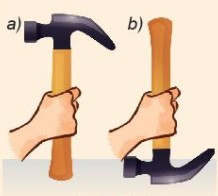
\includegraphics[scale=1]{../figs/VN10-2022-PH-TP017-1.jpg}
		\end{center}
		\begin{enumerate}[label=\alph*)]
			\item Đập mạnh cán búa xuống đất như hình a.
			\item Đập mạnh đầu búa xuống đất như hình b.
		\end{enumerate}
	}
	
	\hideall{
		
		Cả 2 cách đều được. 
		
		Nhưng nên chọn cách a vì khi đạp cán búa xuống đất thì lực tác dụng lên cán búa sẽ có hướng đi lên khi tác dụng vào búa thì vì do quán tính thì búa sẽ rơi xuống phía dưới theo hướng ngược lại với hướng của lực tác dụng lên cán. Thì như vậy, đầu búa sẽ dễ tra vào cán hơn.
	}
		\item \mkstar{1}
	
	{
		Tại sao máy bay khối lượng càng lớn thì đường băng phải càng dài?
	}
	
	\hideall{
		
		Vì máy bay có khối lượng quá lớn, lại bay với tốc độ rất cao nên muốn hạ cánh và dừng lại máy bay cần đường băng dài, thời gian hãm trên đường băng lâu hơn.
	}
		\item \mkstar{1}
	
	{
		Hãy chỉ ra các cặp lực và phản lực trong hai trường hợp sau:
		\begin{enumerate}[label=\alph*)]
			\item Quyển sách nằm yên trên mặt bàn hình a.
			\item Dùng búa đóng đinh vào gỗ hình b.
		\end{enumerate}
		\begin{center}
			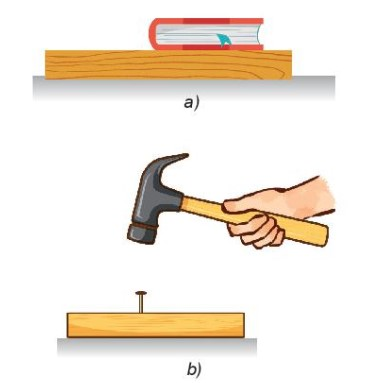
\includegraphics[scale=1]{../figs/VN10-2022-PH-TP017-3.jpg}
		\end{center}
	}
	
	\hideall{
		\begin{enumerate}[label=\alph*)]
			\item Lực là của lực hút trái đất, phản lực là lực cản của mặt bàn.
			\item Lực do búa tác dụng lên đinh và phản lực của đinh tác dụng vào búa.
		\end{enumerate}
	}
		\item \mkstar{1}
	
	{
		
		Một ô tô chuyển động trên mặt đường, nếu lực do ô tô tác dụng lên mặt đường có độ lớn bằng lực mà mặt đường đẩy ô tô thì tại sao chúng không "khử nhau"?
		\begin{center}
			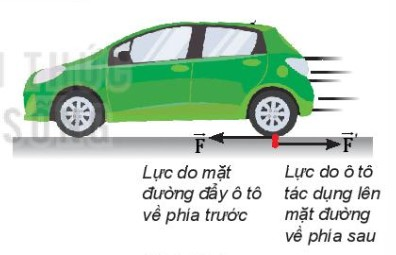
\includegraphics[scale=0.6]{../figs/VN10-2022-PH-TP017-4.jpg}
		\end{center}
	}
	
	\hideall{
		
		Vì căn bản 2 lực này tác dụng lên hai vật khác nhau. Lực do ô tô tác dụng lên mặt đường thì lực được đặt ở mặt đường. Lực mà mặt đường đẩy ô tô thì được đặt vào ô tô.
	}
		\item \mkstar{1}
		
		{
		Trong trò chơi thổi viên bi, mỗi bạn sử dụng một ống bơm khí từ vật liệu đơn giản như hình, thổi khí vào viên bi được đặt trên ray định hướng. Người chơi sẽ chiến thắng khi thổi viên bi đi xa hơn sau ba lần. Hãy sử dụng định luật II Newton giải thích làm thế nào để có thể chiến thắng trò chơi này.
		\begin{center}
			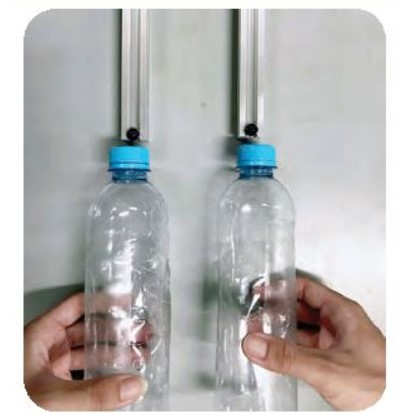
\includegraphics[scale=0.6]{../figs/VN10-2022-PH-TP017-5.jpg}
		\end{center}
		}
		
		\hideall{
			
			Áp dụng định luật II Newton, ta có lực càng lớn thì gia tốc càng lớn, vật sẽ càng đi được xa. Ta bóp ở cuối chai thì sẽ tạo ra lực lớn.
		
		}
			\item \mkstar{1}
		
		{
			Xét trường hợp con ngựa kéo xe như hình. Khi ngựa tác dụng một lực kéo lên xe, theo định luật III Newton sẽ xuất hiện một phản lực có cùng độ lớn nhưng ngược hướng so với lực kéo. Vậy tại sao xe vẫn chuyển động về phía trước? Giải thích hiện tượng.
			\begin{center}
				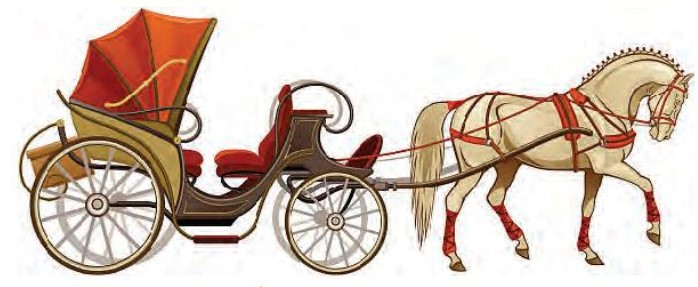
\includegraphics[scale=0.6]{../figs/VN10-2022-PH-TP017-6.jpg}
			\end{center}
		}
		
		\hideall{
			
			Do hai lực tác dụng vào hai vật (xe, ngựa) khác nhau nên hai lực này không thể triệt tiêu nhau lẫn nhau được nên xe vẫn chuyển động về phía trước.
			
			
		}
		\item \mkstar{2}
	
	{
		
		Dưới tác dụng của hợp lực $\SI{20}{N}$, một chiếc xe đồ chơi chuyển động với gia tốc $\SI{0,4}{m/s}^2$. Dưới tác dụng của hợp lực $\SI{50}{N}$, chiếc xe sẽ chuyển động với gia tốc bao nhiêu?
	}
	
	\hideall{
		
		Dưới tác dụng của hợp lực $\SI{50}{N}$, chiếc xe sẽ chuyển động với gia tốc
		
		$$m=\dfrac{F_1}{a_1} = \dfrac{F_2}{a_2} \Rightarrow a_2 = \dfrac{F_2a_1}{F_1} = \SI{1}{m/s}^2.$$
		
	}
	\item \mkstar{2}
	
	
	{Cho đồ thị biểu diễn mối liên hệ giữa các lực tác dụng lên một vật và gia tốc gây ra tương ứng. Khối lượng của vật là bao nhiêu?
		
		\begin{center}
			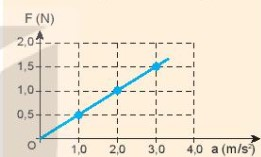
\includegraphics[scale=1]{../figs/VN10-2022-PH-TP017-2.jpg}
		\end{center}
	}
	
	\hideall
	{	
		
		Khối lượng của vật là
		
		$$m = \dfrac{F_1}{a_1} = \dfrac{F_2}{a_2} = \dfrac{F_3}{a_2} = \dfrac{\text{0,5}}{\text{1,0}} = \dfrac{\text{1,0}}{\text{2,0}} =\dfrac{\text{1,5}}{\text{3,0}} = \SI{0,5}{kg}.$$
		
	}
	\item \mkstar{2}
	
	
	{Một quả bóng khối lượng $\SI{0,5}{kg}$ đang nằm yên trên mặt đất. Một cầu thủ đá bóng với một lực $\SI{250}{N}$. Thời gian châm tác dụng vào bóng là $\SI{0,02}{s}.$ Quả bóng bay đi với tốc độ bao nhiêu?
	}
	
	\hideall
	{
		Lực làm quả bóng chuyển động chỉ gồm lực do chân của cầu thủ.
		
		Áp dụng định luật II Newton, chiếu lên phương chuyển động (quả bóng chuyển động cùng phương với lực tác dụng), gia tốc của bóng là:
		
		$$a = \dfrac{F}{m} = \SI{500}{m/s}^2.$$
		
		Vận tốc của quả bóng là
		
		$$a = \dfrac{\Delta v}{\Delta t} \Rightarrow v - v_0 = v = a \Delta t = \SI{10}{m/s}\ (v_0 = 0).$$
		
		
	}
	\item \mkstar{2}
	
	
	{Một xe tải khối lượng 1 tấn, sau khi khởi hành được $10\ \text s$ đạt vận tốc $18\ \text{km/h}$. Biết lực cản mà mặt đường tác dụng lên xe là $500\ \text N$. Tính lực phát động của động cơ.
	}
	
	\hideall
	{	Gia tốc của xe:
		\[a = \dfrac{v-v_0}{\Delta t} = \dfrac{1}{2}\ \text{m/s}^2\]
		
		Mà $F-F_\text c = ma \Rightarrow F = F_\text c + ma = 500 + 500 = 1000\ \text N$
	}
	\item \mkstar{3}
	
	
	{Một ô tô có khối lượng 1 tấn đang chuyển động với $v=54\ \text{km/h}$ thì tắt máy, hãm phanh, chuyển động chậm dần đều. Biết độ lớn lực hãm $3000\ \text N$. Xác định quãng đường xe đi được cho đến khi dừng lại.
	}
	
	\hideall
	{Chọn chiều dương là chiều chuyển động, gốc thời gian lúc bắt đầu hãm phanh.
		
		Áp dụng định luật II Newton:
		\[ \vec a = \dfrac {\vec F}{m} \Rightarrow a=\dfrac{F}{m} = \dfrac{-3000}{1000} = -3\ \text{m/s}^2\]
		
		Mà $v^2 - v_0 ^2 = 2as$, suy ra $s=37,5\ \text m$.
	}

\end{enumerate}